\documentclass[12pt,a4paper,titlepage,headinclude,bibtotoc]{scrartcl}

%---- Allgemeine Layout Einstellungen ------------------------------------------

% Für Kopf und Fußzeilen, siehe auch KOMA-Skript Doku
\usepackage[komastyle]{scrpage2}
\pagestyle{plain}
\setheadsepline{0.5pt}[\color{black}]
\automark[section]{chapter}


%Einstellungen für Figuren- und Tabellenbeschriftungen
\setkomafont{captionlabel}{\sffamily\bfseries}
\setcapindent{0em}


%---- Weitere Pakete -----------------------------------------------------------
% Die Pakete sind alle in der TeX Live Distribution enthalten. Wichtige Adressen
% www.ctan.org, www.dante.de

% Sprachunterstützung
\usepackage[ngerman]{babel}

% Benutzung von Umlauten direkt im Text
% entweder "latin1" oder "utf8"
\usepackage[utf8]{inputenc}

% Pakete mit Mathesymbolen und zur Beseitigung von Schwächen der Mathe-Umgebung
\usepackage{latexsym,exscale,stmaryrd,amssymb,amsmath}


\usepackage[nointegrals]{wasysym}
\usepackage{eurosym}

% Anderes Literaturverzeichnisformat
%\usepackage[square,sort&compress]{natbib}
\usepackage{hyperref}
% Für Farbe
\usepackage{color}
\usepackage{graphicx}
\usepackage{wrapfig}
\usepackage{subfigure}

% Caption neben Abbildung
\usepackage{sidecap}


% Befehl für "Entspricht"-Zeichen
\newcommand{\corresponds}{\ensuremath{\mathrel{\widehat{=}}}}
% Befehl für Errorfunction
\newcommand{\erf}[1]{\text{ erf}\ensuremath{\left( #1 \right)}}


%Fußnoten zwingend auf diese Seite setzen
\interfootnotelinepenalty=1000

%Für chemische Formeln (von www.dante.de)
%% Anpassung an LaTeX(2e) von Bernd Raichle
\makeatletter
\DeclareRobustCommand{\chemical}[1]{%
  {\(\m@th
   \edef\resetfontdimens{\noexpand\)%
       \fontdimen16\textfont2=\the\fontdimen16\textfont2
       \fontdimen17\textfont2=\the\fontdimen17\textfont2\relax}%
   \fontdimen16\textfont2=2.7pt \fontdimen17\textfont2=2.7pt
   \mathrm{#1}%
   \resetfontdimens}}
\makeatother
\usepackage{textcomp}
\usepackage{upgreek}
%\begin{document}
%$\upmu$
%\end{document}
%Honecker-Kasten mit $$\shadowbox{$xxxx$}$$
\usepackage{fancybox}

%SI-Package
\usepackage{siunitx}

%keine Einrückung, wenn Latex doppelte Leerzeile
\parindent0pt

%Bibliography \bibliography{literatur} und \cite{gerthsen}
%\usepackage{cite}
\usepackage{babelbib}
\selectbiblanguage{ngerman}

\usepackage{siunitx}
%\begin{document}
 % \SI{1.55}{\micro\metre}
\sisetup{math-micro=\text{µ},text-micro=µ}
\usepackage{amsmath}

\usepackage[verbose]{placeins}
%für \FloatBarrier

\begin{document}

\begin{titlepage}
\centering
\textsc{\Large Physikalisch- Chemisches Grundpraktikum\\[1.5ex] Universität Göttingen}

\vspace*{0.5cm}

\rule{\textwidth}{1pt}\\[0.5cm]
{\huge \bfseries
  Versuch 1: \\[1.5ex]
  Molare Wärmekapazität von Festkörpern }\\[0.5cm]
\rule{\textwidth}{1pt}

\vspace*{0.5cm}


\begin{Large}
\begin{tabular}{ll}
Durchführende: &  Isaac Maksso, Julia Stachowiak\\
Assistent: & Sven Meyer \\
 Versuchsdatum: & 10.11.2016\\
 Datum der ersten Abgabe: & 17.11.2017\\
\end{tabular}
\end{Large}

\vspace*{0.5cm}


\begin{table}[h!]
\centering
\caption{Ergebnisse des Versuchs.}
\begin{tabular}{c|c|c|c||c|c}
Probe&Temperaturbad&$\text{c}_P^{\text{Exp.}}$ [$\frac{\text{J}}{\text{mol}\cdot\text{K}}$] &$\text{c}_P^{\text{Lit.}}$ [$\frac{\text{J}}{\text{mol}\cdot\text{K}}$] & $<\Theta_D >$ [K]& $<\Theta_{D,Lit.}>$ [K] \\
\hline
Graphit& ZT&4,52 ± 0,053  &8,517& 138$ \cdot 10^2$& 2500950\\
\hline
Zink &ZT& 51,7 ± 0,260 &24,47& 981 & 345\\
\hline
Kupfer &ZT&55,9 ± 0,242 &25,330& 630 &308\\
\end{tabular}
\end{table}
\end{titlepage}


\tableofcontents

\newpage


\section{Experimentelles}
\subsection{Experimenteller Aufbau}

\subsection{Durchführung}
Es wurde 0.4002\;g Silberiodid abgewogen und zu einer Tablette gepresst. Es wurde eine Feststoffkette, wie in Abbildung ... zu sehen ist, aufgebaut und 10\;min mit $\text{N}_2$-Gas umspült. Die Feststoffkette wurde auf 160\;°C hochgeheizt und 45\;min bei einem Strom von 1.2\;mA aufgeladen. Es wurde ab 160\;°C in 5\;°C-Schritten die Spannung gemessen. Ab 175\;°C wurde das Messgerät kurzgeschlossen und die Messung fortgesetzt. 
\section{Auswertung}
\subsection{Messergebnisse}
In der Tabelle 2 sind die Messergebnisse der Elektromotorischenkraft dargestellt.
\begin{table}[h!]
\centering
\caption{Messergebnisse des Versuchs.}
\begin{tabular}{c|c||c|c}
T/\;K & EMK/\;V &T/\;K & EMK/\;V\\ 
\hline
433.7 & 0,2889 &   488.15 &0,2860\\ 
438.5 & 0,2871 & 493.15&0,2868 \\
443.25 & 0,2772 &  498.15&0,2877\\
448.15 & 0,2782 & 503.15& 0,2885\\
453.15 &0,2792 & 508.15 &0,2893\\
458.15 & 0,2803 & 513.15 &0,2900\\
463.15 &0,2814 & 518.15 &0,2903\\
468.15 &0,2826 & 523.15&0,2916\\
473.15 &0,2838 & 528.15 & 0,2923\\
478.15 & 0,2844 & 533.15& 0,2933\\
483.15 & 0,2852 &&\\
\end{tabular} 
\end{table}
\FloatBarrier
\subsection{$\Delta_R G$(T) gegen T}
Die freie Reaktionsenergie $\Delta_R G$ lässt sich nach Gl. 1 erechnen:
\begin{align}
\Delta_R G &= - z F \Delta E 
\end{align}
$\Delta E$ berechnet sich folgendermaßen:
\begin{align}
\Delta E &= \Delta E^0 + z\cdot F \cdot \frac{\text{a}(\text{Ag}_2\text{Se})}{\text{a}(\text{Ag})^2\cdot\text{a}(\text{Se})}\\
\Delta E &= \Delta E^0 + R\cdot T\cdot \text{ln}(\frac{1}{1^2\cdot1})\\
\Delta E &= \Delta E^0 + RT \cdot \text{ln}(1)\\
\Delta E &= \Delta E^0 \\
\end{align}
Da die Aktivität von Feststoffen 1 ist, fällt der logorithmische Term weg und Die EMK ist gleich dem Standardelektrodenpotential.\\
Die Werte für $\Delta_R G$ (T) sind in der Tabelle~3 dargestellt.
\begin{table}[h!]
\centering
\caption{Ergebnisse für $\Delta_R G$.}
\begin{tabular}{c|c||c|c}
T/\;K & $\Delta_R G$/\;$\frac{\text{kJ}}{\text{mol}}$ &T/\;K & $\Delta_R G$/\;$\frac{\text{kJ}}{\text{mol}}$\\ 
\hline
433.7 & -55.75 &488.15 & -55.19 \\ 
438.5 & -57.33 & 493.15& -55.52 \\
443.25 & -55.42 &  498.15& -55.67\\
448.15 & -53.68 & 503.15&  -55.83\\
453.15 & -53.88 & 508.15 & -55.96\\
458.15 & -54.09 & 513.15 & -56.12\\
463.15 & -54.30 & 518.15 & -56.12\\
468.15 & -54.53 & 523.15& -56.27\\
473.15 & -54.77 & 528.15 & -56.41\\
478.15 & -54.88 & 533.15& -56.60\\
483.15 & -55.04 &&\\
\end{tabular} 
\end{table}
\FloatBarrier
Der Fehler der freien Reaktionsenthalpie $\Delta(\Delta_R G)$  wird mittels Fehlerfortpflanzung berechnet. Bei den ersten drei Messungen schwankte die Anzeige auf dem Voltometer. Es wurde die Schwankung als Fehler notiert. Ab der veriten Messung konnte die EMK ohne Schwankungen abgelesen werden. Der Fehler wird 0,0005 V:
\begin{align}
\Delta(\Delta_R G)= \sqrt{(-z\cdot F \cdot \Delta(\Delta E))^2}
\end{align}
\begin{table}[h]
\centering
\caption{Fehler für $\Delta_R G$.}
\begin{tabular}{c|c|c}
Temperatur/ K & $\Delta(\Delta E)$/ V & $\Delta(\Delta_R G)$/ J \\
\hline
458.15 &  0.005 &  0.1  \\
46315 & 0.003   & 0.06 \\
468.15 & 0.003  & 0.06 \\
473.15 & 0.0005& 0.01 \\
478.15 & 0.0005& 0.01 \\
483.15 & 0.0005& 0.01 \\
488.15 & 0.0005& 0.01 \\
493.15 & 0.0005& 0.01 \\
498.15 & 0.0005& 0.01 \\
503.15 & 0.0005& 0.01 \\
508.15 & 0.0005& 0.01 \\
513.15 & 0.0005& 0.01 \\
518.15 & 0.0005& 0.01 \\
523.15 & 0.0005& 0.01 \\
528.15 & 0.0005& 0.01 \\
533.15 & 0.0005& 0.01 \\
\end{tabular}
\end{table}
\FloatBarrier
\subsection{$\Delta E$ gegen T}
Es wurden die Werte für $\Delta E$ und T aus Tabelle~2 mit den Fehlern aus für $\Delta E$ aus Tabelle~3 aufgetragen in Abbildung~1 aufgetragen. Die Temperatur wurde als fehlerfrei angenommen, da diese nach einer langen Aufheizphase durch kleine Temperaturerhöhungen mittels Thermodingsbums eingestellt wurde. Es wurden bei der linearen Regression die ersten drei Messpunkte nicht eingefügt, da sie sehr stark von den folgenden Messwerten abweichen. 
\begin{figure}[h]
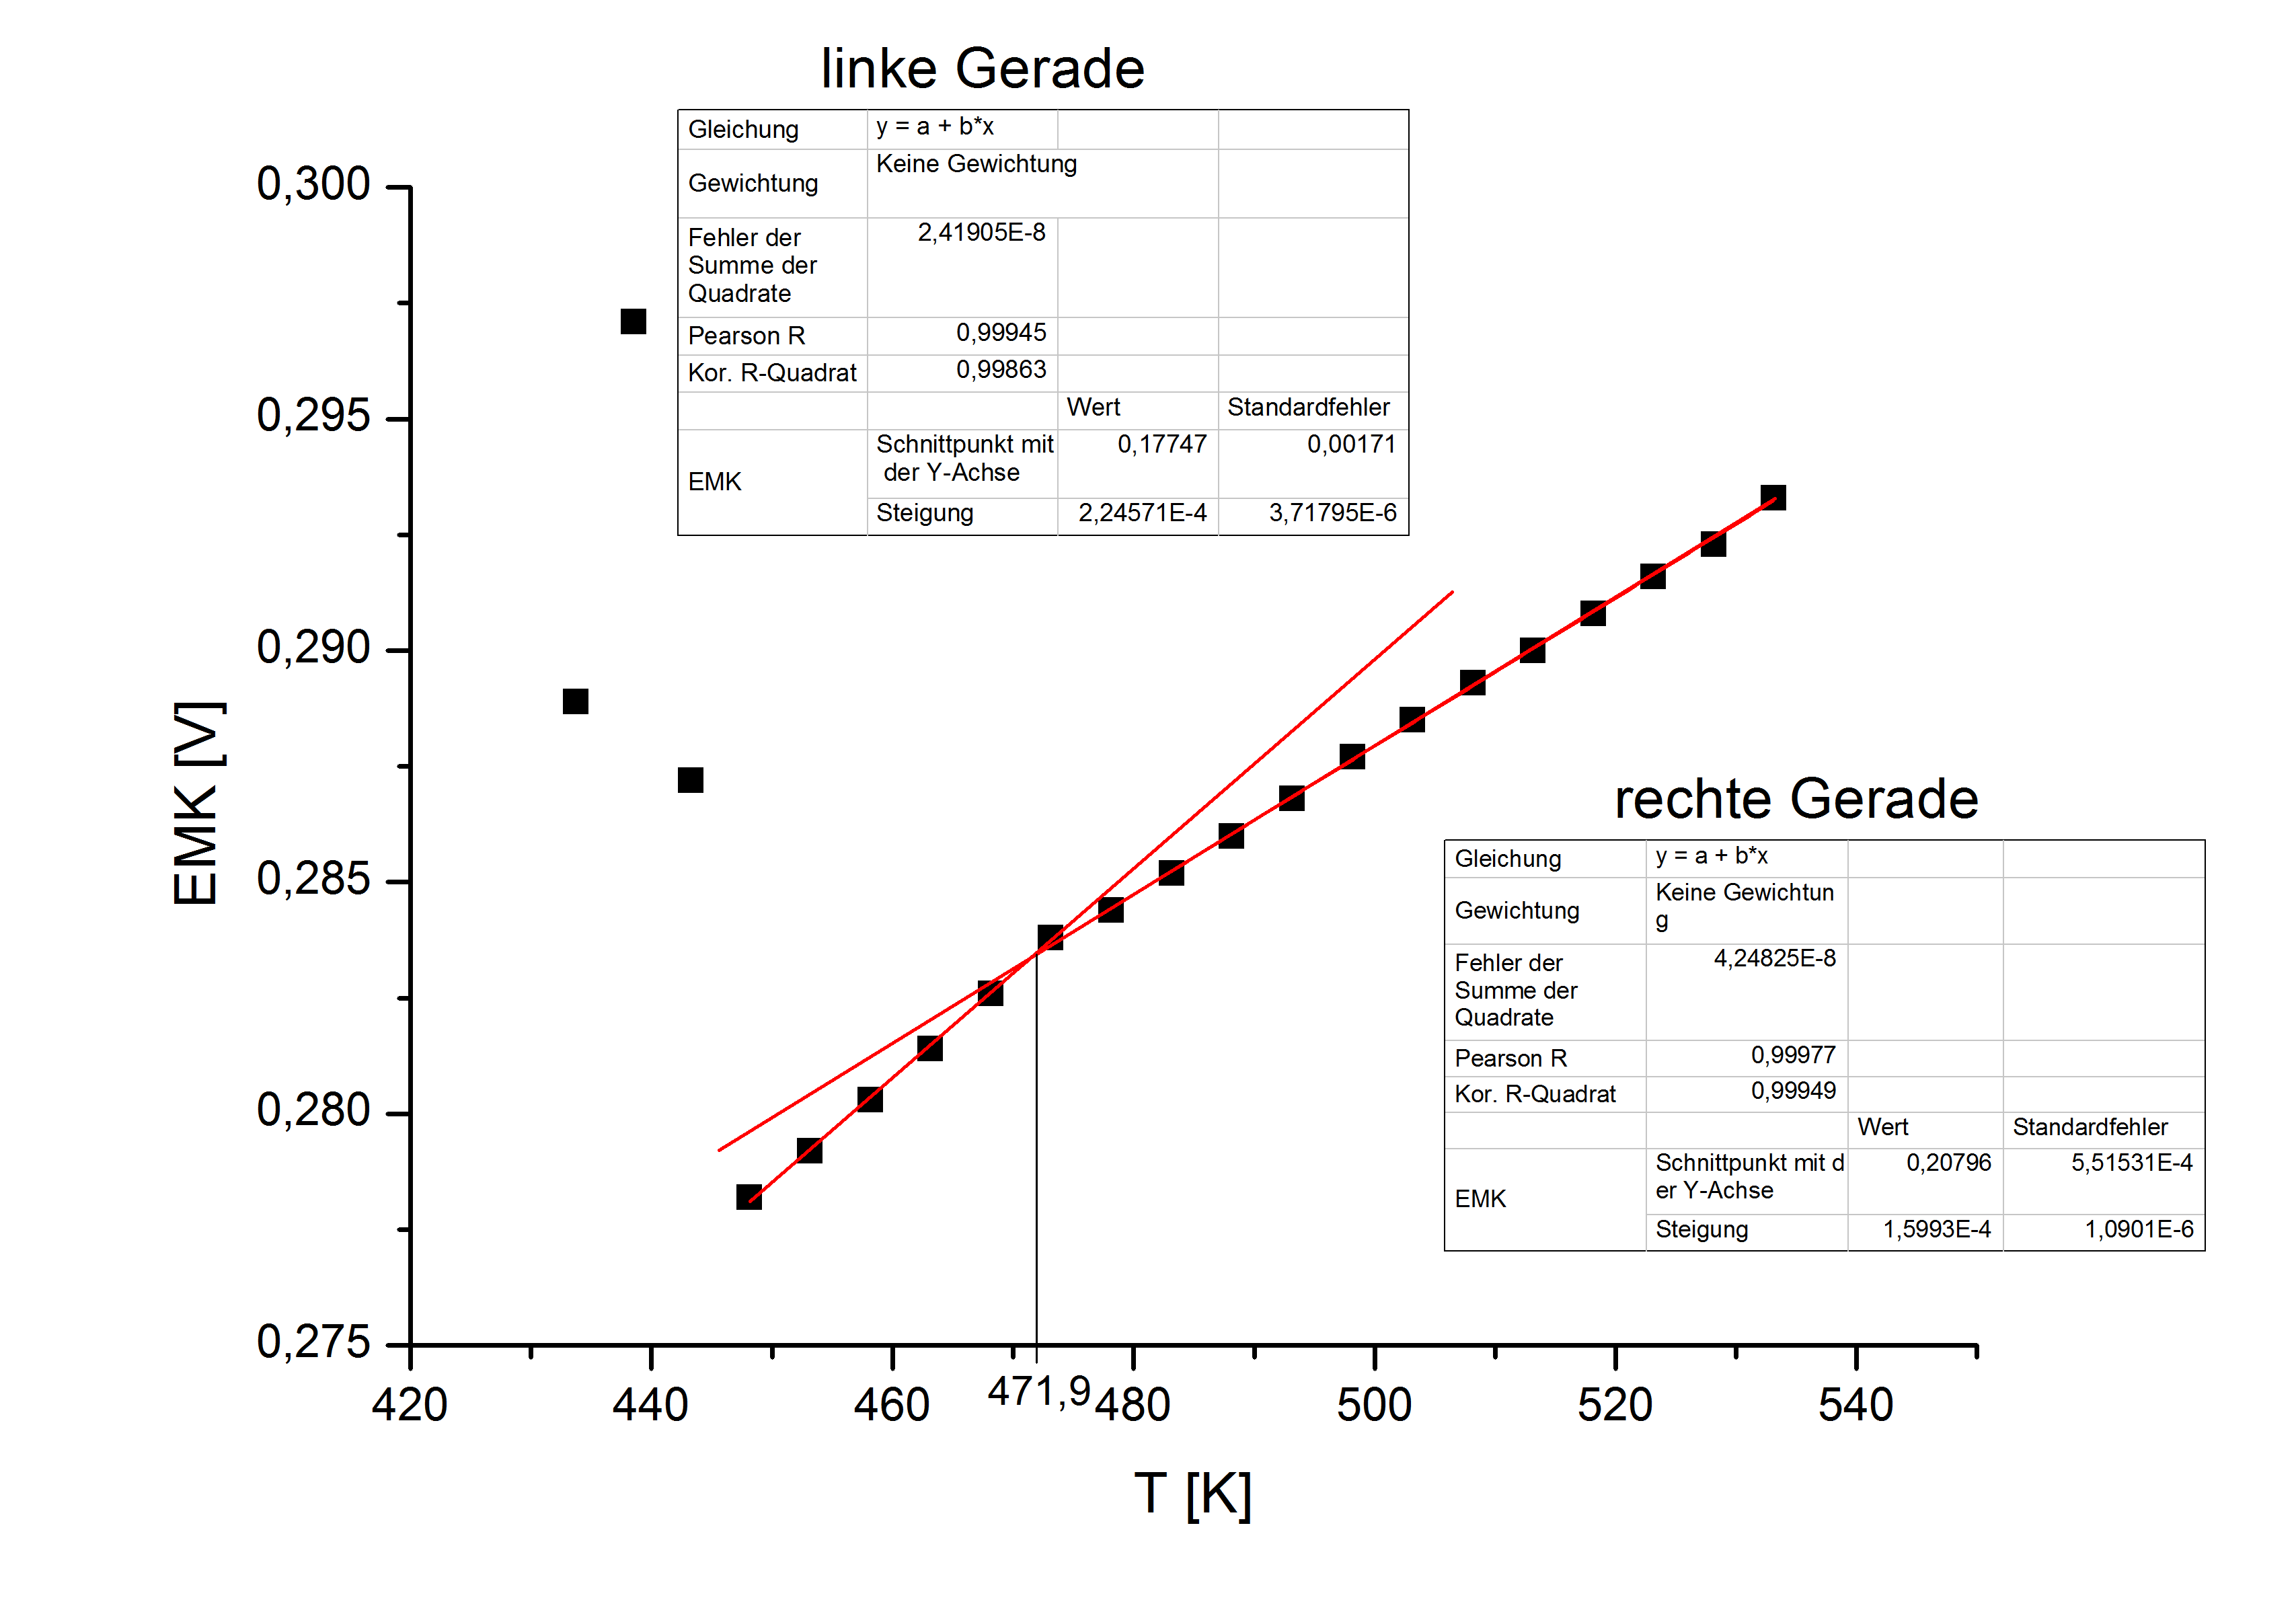
\includegraphics[width=13.5cm]{EMK_gegen_T.png}
\caption{$\Delta E$ gegen T.}
\end{figure} 
Die negative Ableitung der freien Reaktionsentalpie nach der Temperatur ist gleich der Reaktionsentropie. Durch einsetzen der Gleichung~1 wird die Formel zur Berechnung der Reaktionsentropie erhalten. 
\begin{align}
\Delta_R S &= -(\frac{\partial \Delta_R G}{\partial T})\\
&= z \cdot F \cdot (\frac{\partial \Delta E}{\partial T})\\
&= z \cdot F \cdot m \\
\Delta_R S_{\text{m}} &= 2 \cdot 9.6485 \cdot 10^4\;\text{As} \cdot 2.24 \cdot 10^{-4}\;\frac{\text{V}}{\text{K}}\\
&= 43.3\;\frac{\text{J}}{\text{K}}\\
\Delta_R  S_{\text{l}} &= 2 \cdot  9.6485 \cdot 10^4\;\text{As} \cdot 1.60 \cdot 10^{-4}\;\frac{\text{V}}{\text{K}}  \\
&= 30.9\;\frac{\text{J}}{\text{K}}\\
\end{align}
Der Fehler der Reaktionsentropie lässt sich mittels Fehlerfortpflanzung berechnen. Der Fehler der Steigung wird hierbei aus dem Auswertungsblatt des Programms $Origin 8.5 G$ entnommen. 
\begin{align}
\Delta(\Delta_R  S)&= \sqrt{(z\cdot F \cdot \Delta m)^2}\\
\Delta(\Delta_R  S_{\text{m}})&= \sqrt{(2\cdot 9.6485 \cdot 10^4\;\text{As} \cdot 0.04 \cdot 10^{-4}\;\frac{\text{V}}{\text{K}})^2}\\
&= 0.7 \;\frac{\text{J}}{\text{K}}\\
\Delta(\Delta_R  S_{\text{l}})&= \sqrt{(2\cdot 9.6485 \cdot 10^4\;\text{As} \cdot 0.01\cdot 10^{-4}\;\frac{\text{V}}{\text{K}})^2}\\
&= 0.2\;\frac{\text{J}}{\text{K}}
\end{align}
\section{Bestimmung der Reaktionsenthalpie}
\section{Auftragung nach Vant'Hof}
\section{Bestimmung der Umwandlungsenthalpie und Umwandlungsentropie}
\section{Schmelzpunktbestimmung}
\section{Diskussion}
\newpage
\section{Literaturverzeichnis}
1\quad Eckhold, Götz: \emph{Praktikum I zur Physikalischen Chemie}, Institut für Physikalische Chemie, Uni Göttingen, \textbf{2014}.

\vspace{0,5 cm}
2 \quad Eckhold, Götz: \emph{Statistische Thermodynamik}, Institut für Physikalische Chemie, Uni Göttingen, \textbf{2012}.

\vspace{0,5cm}
3 \quad Eckhold, Götz: \emph{Chemisches Gleichgewicht}, Institut für Physikalische Chemie, Uni Göttingen, \textbf{2015}.\\

\end{document}


	